The process of data collection is a critical component in the development of any machine learning model. The quality and relevance of the data collected directly influence the performance and effectiveness of the final model. In the context of autonomous driving, the data collection process becomes even more crucial due to the complexity and variability of real-world driving scenarios.

In this chapter, we describe the creation of CARLA-NAV, the meta-dataset that supports the language-guided navigation approach developed in this thesis.\footnote{Parts of this chapter appear in Jain et al., \textit{Ground then Navigate: Language-guided Navigation in Dynamic Scenes}, IEEE ICRA 2023~\cite{jain2023ground}.} We began with Grand Theft Auto V (GTA V) as an initial data collection environment, then switched to the research-oriented CARLA simulator~\cite{dosovitskiy2017carla}. We also explain our shift from predicting steering, acceleration, and brake values to predicting segmentation maps for navigation, detail the observer--navigator--verifier annotation protocol, and summarize dataset statistics and challenges.

\section{Introduction}

The ability to navigate based on linguistic descriptions of the environment is a remarkable human capability, a direct consequence of associating visual elements with their linguistic descriptions. Referring Expression Comprehension (REC) and Referring Image Segmentation (RIS) aim to localize visual objects based on linguistic descriptions~\cite{rohrbach2016grounding,hu2016segmentation}. However, these localizations are not directly usable for navigation, as they do not answer ``which region'' on the road to navigate to. Referring Navigable Regions (RNR)~\cite{Rufus_2021} was proposed to localize navigable regions in a static front-camera image corresponding to a linguistic command.

While single image-based visual grounding methods showcase the ability of neural models to correlate visual and linguistic data, they are limited in several ways. They are trained on carefully paired data, assuming that the region to be grounded is always visible in the frame. They give erroneous output when the region is not currently visible, is occluded, or goes out of frame. Such scenarios are part of everyday language-guided navigation; for instance, in ``Take a right once you see the traffic signal,'' the traffic signal may not be immediately visible.

Another major limitation is that single-image predictions are devoid of temporal context, which is crucial in successful navigation in dynamically changing environments. Finally, since single-image methods are often evaluated on frames from pre-recorded videos, they cannot be validated on their ability to complete an entire episode from start to finish.

Most existing works on language-guided navigation make assumptions that limit applicability in real-world outdoor settings. Indoor methods often assume a fully known environment that can be discretized into a graph~\cite{anderson2018vision,kolve2017ai2}. Outdoor methods such as Touchdown~\cite{Chen2019TOUCHDOWN} allow navigation by choosing from a small discrete action set on pre-recorded street views. This discretization limits fine manoeuvres such as ``park between the two cars on the right.''

To address these limitations, we created CARLA-NAV using the CARLA simulator~\cite{dosovitskiy2017carla}. Combined with a visual grounding-based approach, the dataset allows fine-grained control over the vehicle by enabling navigation to any drivable region on the road. Live language-guided navigation in simulation has prior precedents; our contribution is a continuous-control, region-grounding formulation with dense annotations for outdoor dynamic scenes.

\section{Initial Data Collection with GTA V}

We initially attempted to collect data using Grand Theft Auto V (GTA V) and the DeepGTAV and V-Pilot mods. The game's realistic graphics, diverse urban environments, and dynamic traffic made it an appealing choice for simulating real-world driving conditions. DeepGTAV allows extraction of camera images, vehicle state, and information about other agents in the scene.

Our initial approach was to train a deep learning model to predict steering, acceleration, and brake. However, we encountered several challenges. First, predicting only three continuous controls without sufficient high-level context proved brittle, consistent with observations that end-to-end driving models can struggle without structured guidance~\cite{bansal2018chauffeurnet,Codevilla_Muller_Lopez_Koltun_Dosovitskiy_2018}. Second, supervised learning alone was insufficient without a carefully designed reward if we moved to reinforcement learning, and defining rewards for language-conditioned driving is itself a hard problem~\cite{sutton2018reinforcement,hadfieldmenell2017inverse}. GTA V also did not provide the per-pixel and camera-calibration access needed for dense navigable-region annotation.

Given these challenges, we switched to predicting segmentation masks under supervised learning. Dense mask prediction provides a more interpretable target and a clearer visual representation of what the model believes is navigable~\cite{uricar2021desoiling,hanselmann2022king}. In the next section, we discuss why CARLA made this approach feasible.

\section{Switching to CARLA for Data Collection}

After encountering limitations with GTA V, we switched to CARLA~\cite{dosovitskiy2017carla}, an open-source simulator designed for autonomous driving research. CARLA offers several advantages that made it suitable for our purposes:

\begin{enumerate}
    \item \textbf{Research-oriented control:} CARLA provides flexible control over weather, time of day, and the behaviour of other vehicles and pedestrians, which is crucial for a diverse dataset.
    \item \textbf{Consistent physics:} Vehicle motion and interactions with the environment are more reliable than in a commercial game pipeline.
    \item \textbf{Rich environment state:} Access to 3D object positions, road layout, and sensor metadata supports precise annotation.
    \item \textbf{Camera calibration:} Live camera intrinsics and orientation matrices enable transforming 2D screen coordinates into 3D world coordinates---essential for projecting navigable regions and driving a local planner.
\end{enumerate}

These capabilities allowed us to adopt visual grounding: associating linguistic descriptions of navigable regions with their visual counterparts and predicting a segmentation map that can be used for navigation. This shift would not have been feasible in GTA V due to limited access to internal game data.

\section{Data Collection Methodology}

The data collection process in CARLA was a collaborative effort involving three roles: the observer, the navigator, and the verifier.

\begin{itemize}
    \item \textbf{Observer:} Provides clear linguistic commands based on the current environment state. Commands are generated on-the-fly rather than scripted, capturing natural variation.
    \item \textbf{Navigator:} Drives in CARLA by clicking navigable regions in the front-camera view and follows the observer's command as naturally as possible. A restart option is available for erroneous clicks.
    \item \textbf{Verifier:} Reviews the language command, navigated path, and generated masks, and decides whether the episode is included in the dataset.
\end{itemize}

The 2D screen coordinates clicked by the navigator are transformed into 3D world coordinates using the inverse projective transform with CARLA's camera intrinsic and orientation matrices under a flat-ground assumption. This 3D position is passed to the local planner (CARLA's default planner in our case; the design is modular and can later use planners such as NEAT~\cite{chitta2021neat}). Early collection prototypes also experimented with reading depth from a CARLA depth camera for the clicked pixel; the released CARLA-NAV annotations follow the flat-ground rectangle projection documented below and in the archival paper.

An episode comprises multiple mouse clicks until the final navigable region becomes visible in the front view. Intermediate clicks signify intermediate navigable regions; the last click depicts the final goal region. Mouse clicks are converted into segmentation masks by drawing a $3\mathrm{m} \times 4\mathrm{m}$ rectangle (approximately the size of a car) in the top view, centred at the click, and projecting that rectangle into the front camera. Overall, only language commands and mouse clicks require manual effort; the rest of the annotation process is automated. Early drafts treated intermediate and final regions as two separate segmentation classes to drive stopping; the released dataset and CLIP-family models use a single navigable-region mask, with the area-based stopping rule described in Chapter~\ref{ch:vln}.

For the trajectory prediction task used later for interpretability, we take the 3D position of the vehicle in successive frames and project those positions onto the front-camera image. Trajectory prediction is treated as a dense prediction task and is not quantitatively evaluated.

Figure~\ref{fig:data_pipeline} summarises the collection loop; Figure~\ref{fig:dataset_sample} shows ground-truth annotations for three sampled frames from an episode of CARLA-NAV.

\begin{figure}[ht]
\centering
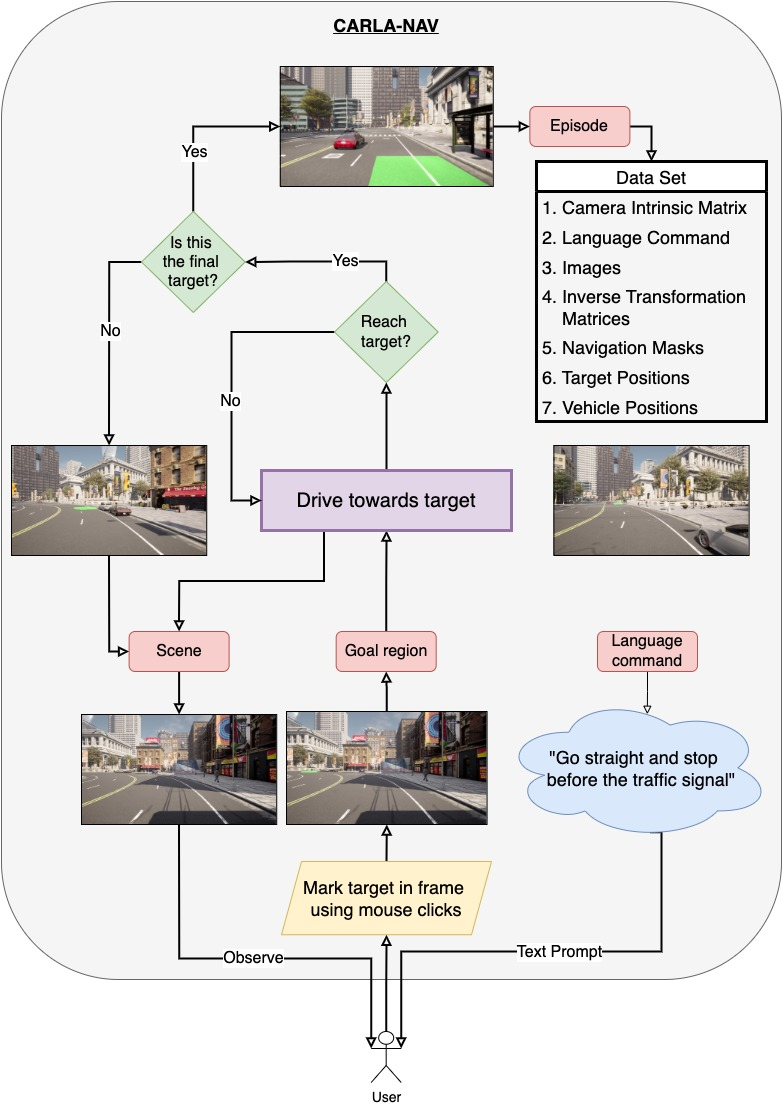
\includegraphics[width=0.85\textwidth]{figures/vln/dataset_pipeline_v4.jpg}
\caption{Pipeline for CARLA-NAV data collection. The user provides a language command and marks successive navigable regions with mouse clicks; the toolkit drives toward each target until the final destination, then stores camera matrices, images, masks, and vehicle/target positions.}
\label{fig:data_pipeline}
\end{figure}

\begin{figure*}[ht]
\centering
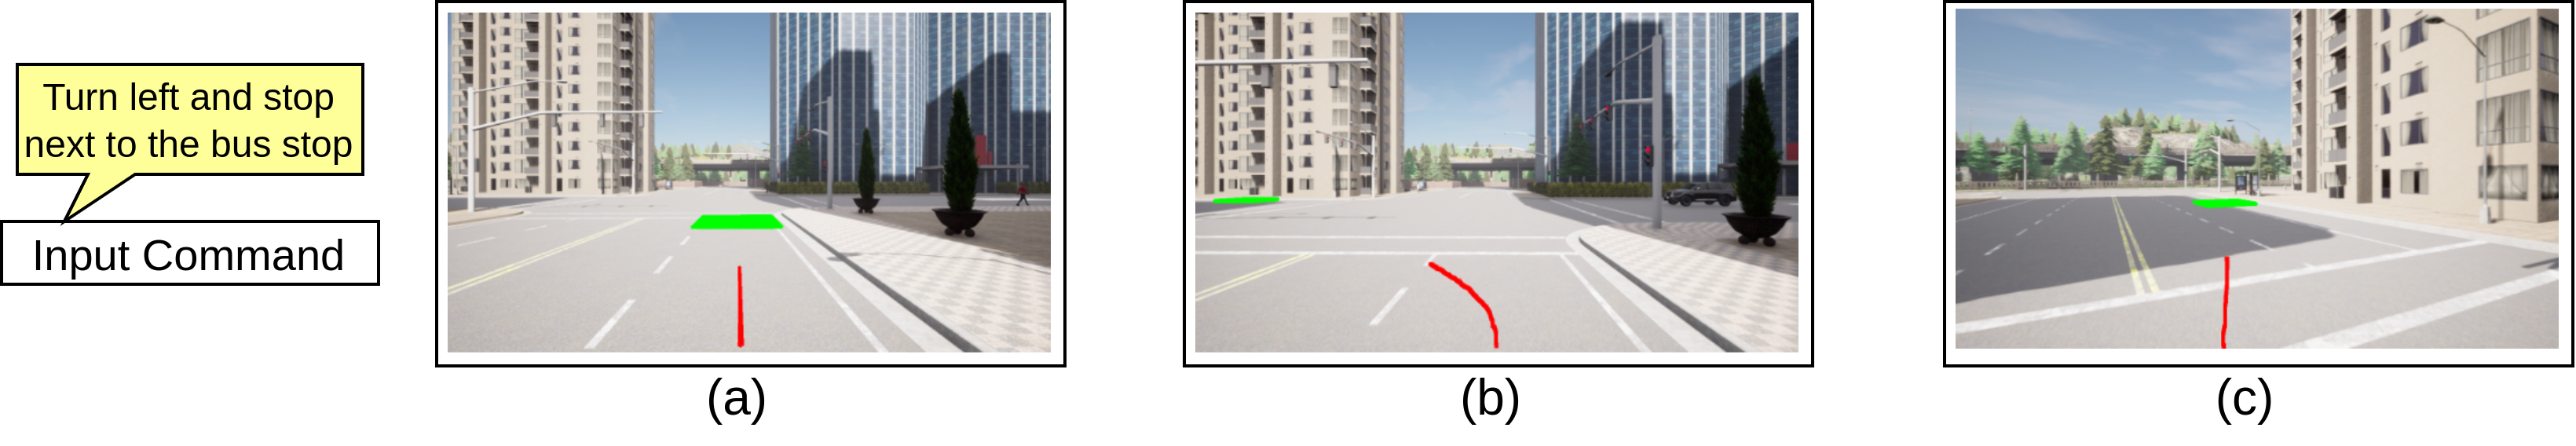
\includegraphics[width=0.98\textwidth]{figures/vln/dataset_sample_v6.png}
\caption{Ground truth annotations of three sampled frames from an episode of the CARLA-NAV dataset. The textual command for the episode is shown on the top. The green rectangle illustrates the navigable region, and the red curve corresponds to the short future trajectory. (a) At the start, the left turn or the final navigable region is not visible, so a straight path is chosen as the intermediate mask; (b) the intermediate mask corresponding to the left turn; (c) the final navigable region (stop next to the bus stop).}
\label{fig:dataset_sample}
\end{figure*}

\section{Dataset Characteristics}

Relative to prior language-guided navigation and grounding datasets surveyed in Chapter~\ref{ch:background} (Table~\ref{table:dataset_comparison}), CARLA-NAV is designed for outdoor dynamic scenes with continuous control and live episode-level evaluation. CARLA-NAV contains episodic data: each episode consists of a language command and the corresponding CARLA video of navigation toward the final goal region described by the command. The ground-truth segmentation mask for each frame corresponds to either the final or an intermediate navigable region. Each frame is additionally annotated with a plausible future trajectory of the vehicle in the next few frames.

The dataset includes video sequences captured in 8 different maps, 14 distinct weather conditions, and a diverse range of dynamically moving vehicles and pedestrians. Language commands contain detailed visual descriptions and describe a wide range of manoeuvres. Commands can have a single manoeuvre (e.g., park behind the black car on the left) or multiple manoeuvres (e.g., take a right turn and park near the bus stand), with a maximum of three manoeuvres.

Table~\ref{table:data_stats} reports core episode statistics. Since each episode contains multiple frames, the overall dataset size is 83,297 frames across all splits. During training we use pre-recorded sequences. During inference on validation and test splits, the vehicle is spawned at the corresponding starting location and navigation is performed live based on network prediction, not on the pre-recorded sequences.

The split sizes evolved during the project: an early draft used 441 train / 25 validation episodes; an intermediate draft used 500 train / 50 validation (with an internal note to split validation into 25/25); the released and archival configuration is 500 / 25 / 34 train/val/test as in Table~\ref{table:data_stats}. The additional nine test episodes relative to a 25/25 split were added before the CLIP-family evaluation reported in Chapter~\ref{ch:vln}.

\begin{table}[ht]
\begin{center}
\begin{tabular}{|c|c|c|c|c|c|}
\hline
Split & \# Episodes & \# Frames & Cmd len. & Clicks & Dist.\ (m) \\ \hline
Train & 500 & 75,010 & 6.92 & 1.94 & 34.18 \\ \hline
Val   & 25  & 3,300  & 6.76 & 2.00 & 37.26 \\ \hline
Test  & 34  & 4,987  & 7.44 & 1.97 & 34.71 \\ \hline
\end{tabular}
\end{center}
\caption{Dataset statistics for CARLA-NAV. Command length, clicks, and distance are averages per episode. Distance is measured along the demonstrated trajectory from spawn to final stop.}
\label{table:data_stats}
\end{table}

\paragraph{Language and manoeuvre diversity.}
Commands mainly consist of up to three subcommands, most having two. Subcommands include turning, going straight, stopping, and parking, and reference pedestrians, infrastructure, road elements, other vehicles, and scenery. A manual audit of the command list yields on the order of $10^2$ unique tokens and a few hundred distinct command strings after lowercasing (many near-paraphrases); we do not claim an exact vocabulary size without a released tokeniser dump. Relative to indoor VLN datasets such as R2R~\cite{anderson2018vision}, whose instructions average on the order of 29 words, CARLA-NAV commands are short (6.9--7.4 words). The language task is therefore substantially simpler than long-horizon indoor instruction following; the difficulty instead lies in dynamic outdoor grounding and continuous control. Chapter~\ref{ch:vln} reports stratified displacement metrics for earlier ViT/Conv3D models under the same target, action, and subcommand taxonomies, and specifies a TC-stratified per-manoeuvre protocol for the CLIP family.

Three distribution figures existed in an earlier draft and must be relocated into \texttt{ms\_thesis\_master/figures/} once recovered. Until then we leave explicit placeholders:

\begin{figure}[ht]
\centering
\fbox{\parbox{0.85\textwidth}{\centering\vspace{1.5cm}\textbf{TODO: Target split in dataset}\\[0.4em]
Recover the figure showing counts / proportions of commands referring to infrastructure vs.\ road/traffic-light vs.\ automobile.\\[0.3em]
{\small (Same taxonomy as Table~\ref{table:target_type} in Chapter~\ref{ch:vln}.)}\vspace{1.5cm}}}
\caption{\textbf{TODO:} Target-type distribution of CARLA-NAV commands. Figure existed in an earlier draft; asset to be relocated into \texttt{figures/}.}
\label{fig:todo_target_split}
\end{figure}

\begin{figure}[ht]
\centering
\fbox{\parbox{0.85\textwidth}{\centering\vspace{1.5cm}\textbf{TODO: Action split in dataset}\\[0.4em]
Recover the figure showing the distribution over primary action verbs (stop / go / take / turn / change / drive / park).\\[0.3em]
{\small (Same taxonomy as Table~\ref{table:action_type} in Chapter~\ref{ch:vln}.)}\vspace{1.5cm}}}
\caption{\textbf{TODO:} Action-verb distribution of CARLA-NAV commands. Figure existed in an earlier draft; asset to be relocated into \texttt{figures/}.}
\label{fig:todo_action_split}
\end{figure}

\begin{figure}[ht]
\centering
\fbox{\parbox{0.85\textwidth}{\centering\vspace{1.5cm}\textbf{TODO: Number of components in dataset}\\[0.4em]
Recover the histogram of subcommands (components) per episode (1 / 2 / 3).\\[0.3em]
{\small Example: ``do this and park near this'' counts as 2.}\vspace{1.5cm}}}
\caption{\textbf{TODO:} Subcommand-count distribution of CARLA-NAV episodes. Figure existed in an earlier draft; asset to be relocated into \texttt{figures/}.}
\label{fig:todo_subcommand_split}
\end{figure}

\paragraph{Maps and weather.}
Episodes span eight CARLA maps and fourteen weather presets (clear, cloudy, wet, sunset, and night variants). Under the default protocol, episodes are shuffled so that maps and weathers appear in all of train, validation, and test in roughly balanced proportions. This design maximises diversity within each small split, but it is \emph{not} a held-out-map protocol: layout memorisation remains possible. The map-unseen evaluation contract is defined in Chapter~\ref{ch:vln}.

\paragraph{Mask annotation coarseness.}
Ground-truth navigable regions are $3\mathrm{m}\times 4\mathrm{m}$ rectangles projected from mouse clicks under a flat-ground assumption. This is a coarse proxy for the true drivable surface: the rectangle may overlap kerbs or undershoot wide parking gaps, and slope transitions introduce projective error (listed below). We treat these masks as supervision for learning \emph{approximate} goal regions rather than pixel-perfect road segmentation, and interpret quantitative mask-conditioned metrics accordingly.

\section{Data Collection Challenges}

We encountered several practical challenges during data collection:

\begin{enumerate}
    \item \textbf{Asynchronous simulation:} CARLA operates asynchronously, so the simulator does not wait for annotation code to finish before advancing. Careful synchronization was required so that frames being annotated matched the displayed state.
    \item \textbf{Slopes:} Transforming 2D screen coordinates into 3D world coordinates assumes a flat ground plane. Transitions from slopes to flat surfaces introduced inaccuracies that required special handling.
    \item \textbf{Split contamination:} Given the finite CARLA maps, similar scenarios can appear across train, validation, and test splits. Shuffling episodes and randomising spawn locations diversifies each split but \emph{does not} hold out maps; a model may still exploit shared layout. Chapter~\ref{ch:vln} therefore defines a map-unseen protocol as the stricter evaluation target.
    \item \textbf{Subjectivity:} Different observers and navigators may interpret the same command differently. Role rotation and verifier checks reduced individual bias.
\end{enumerate}

\section{Data Collection Team and Conclusion}

The CARLA-NAV dataset was curated collaboratively. Annotation roles (observer, navigator, verifier) were rotated among the candidate, Amogh Tiwari, and Kanishk Jain (co-first author of the corresponding ICRA publication~\cite{jain2023ground}). KV~Aditya Srivatsa assisted with early data-collection tooling. Dr.~Vineet Gandhi provided more complex linguistic commands and acted as a verifier in ambiguous cases. A fuller contribution statement appears under Related Publications.

In conclusion, CARLA-NAV provides a diverse set of language-guided outdoor navigation episodes with dense navigable-region and trajectory annotations. The dataset and collection toolkit form the foundation for the multi-task network and live-navigation experiments presented in Chapter~\ref{ch:vln}.
